\twocolumn
\chapter{一元函数微分学}

\begin{definition}
    \label{def:single-order-derivative}
    The derivative of a function $f$ at a number $a$, denoted by $f'(a)$, is 
    \begin{align}
        f'(x_0) &= \lim_{\Delta x \to 0} \dfrac{f(x_0+\Delta x) - f(x_0)}{\Delta x} \\
                &= \lim_{x \to x_0} \dfrac{f(x) - f(x_0)}{x - x_0}
    \end{align}
    if any of the limit exists\footnote{See also the definition of limit \ref{def:limit}}.
\end{definition}
参见小节 $\ref{def-limit}$ 可知,仅给出函数某点$n$阶导数值并不能说明$n$阶导函数存在。
故 L'Hospital 法则不能用。反面例题参见 Example \ref{counter-example-of-usage-of-L-Hospital}.

\section{通用技术}
\label{general-technics-single-var-differentiation}

$n$ 阶可导不能保证 $n$ 阶导函数有极限,也不能保证 $n$ 阶导函数连续。

相当一部分题目是和参数有关的,
当参数作为自变量的系数的时候对其的讨论就会变得复杂。
可以先将式子出以参数的所在的因子的另一部分,是的参数单独出来。
请参考 \ref{number-of-roots-question},例题\ref{example-limits-and-varidic-limits-integral-2}.

可导 $\Rightarrow$ 连续,相关求参数的题目可以用这一性质求出,
比如 \cite[quest27]{w660}

$f^{(n)}$ 在 $x = a$ 存在,不代表 $f^{(n)}$ 在 $a$ 的某邻域一定有定义。
这个时候就不能应用L'hospital 法则。

有关梯度,请参考小节\ref{gradient}.

\subsection{周期函数和导数}

周期函数的导数仍然是周期函数,
若该周期函数具有\textbf{奇偶性},
则它的导数的\textbf{奇偶性刚好相反}。

参见 \cite[quest29]{w660}

\section{利用导数定义求极限}

因为导数就是用极限来定义的,因此如果能将要求的极限式子变化为导数的定义形式
则可以应用求导的方法在求极限上。题目无非就是凑导数定义式。

\begin{example}
    \[
        f(-1) = 1, f'(-1) = 2, \, \mbox{求} \lim_{x \to 1 } \dfrac{f(2-3x) - 1}{x-1}
    \]
    首先观察,分子出现了一个 $-1$,恰好就是 $f(-1)$ ,分母不符合要求,但我们可以乘上一个 factor
    凑出我们想要的式子:
    \begin{align*}
        \mbox{LHS} &= \lim_{x \to 1 } \dfrac{f(-1+\overbrace{3(1-x)}^{\Delta \to 0}) -
             f(-1)}{\underbrace{3(1-x)}_{\Delta \to 0}} \cdot \dfrac{3(1-x)}{x-1} \\
             &= f'(-1) \cdot \lim_{x \to 1} \dfrac{3(1-x)}{x-1} = -6
    \end{align*}
\end{example}
本题还可以按照题目给的条件:$f(-1) = 1, f'(-1) = 2$ 直接给出一个满足条件的简单函数并带入求值,
比如 $f(x) = 2x+3$。
适合选择填空。
注意上面的 $\Delta$ 只要能够 $\to 0$ 就可以。

\section{利用导数定义求导数}

略。

\section{利用导数定义判断函数可导性}

略。

\section{导数的几何意义}

\subsection{求切线}

求切线就注意一点,函数值和该点导数都应该相同,不能仅导数相同。

\section{复合函数求导法}

\subsection{函数奇偶性辅助解题}

比如\footnote{对数运算法则请参考节\ref{logrithemic}.}
\[
    f(x) = \ln(x+\sqrt{1+x^2})
\]
求 $f''(x)$.
这种题目直接使用符合函数求导法则不是很方便,
在做题之前可先观察函数类型,可以发现本函数
是\textbf{奇函数},因此麦克劳林公式展开\footnote{参考小节\ref{tylor}}中,没有偶次导数项。
因此二阶导数为 0.

Tylor 公式的一般形式:
\begin{equation*}
    f(x)=\sum_{i=0}^{n}{\frac{f^{(i)}(x_0)}{i!}(x-x_0)^i}+R_n(x)
\end{equation*}

The reason the second-order derivative at the origin point of an odd function is typically 0 relates to the symmetry properties of odd functions. An odd function is one for which $f(-x) = -f(x)$ for all $x$ in its domain. This property implies that the function is symmetric with respect to the origin.

\subsubsection{Examples of odd functions and their second-order derivatives at the origin}
\begin{enumerate}
    \item The Cubic Function ($f(x) = x^3$):
        \begin{itemize}
            \item $f(x) = x^3$ is an odd function.
            \item The first derivative is $f'(x) = 3x^2$, which is an even function.
            \item The second derivative is $f''(x) = 6x$, which evaluated at the origin ($x = 0$) is $f''(0) = 0$.
        \end{itemize}
    \item Sine Function ($f(x) = sin(x)$):
        \begin{itemize}
            \item The sine function, $\sin(x)$, is an odd function.
            \item The first derivative is $f'(x) = \cos(x)$, which is an even function.
            \item The second derivative is $f''(x) = -\sin(x)$, and when evaluated at the origin ($x = 0$), it's $f''(0) = 0$.
        \end{itemize}
    \item Linear Odd Function ($f(x) = 2x$):
        \begin{itemize}
            \item A simple linear function like $f(x) = 2x$ is an odd function.
            \item The first derivative is a constant, $f'(x) = 2$, which is even.
            \item The second derivative is $f''(x) = 0$, and when evaluated at the origin, it's $f''(0) = 0$.
        \end{itemize}
    \item Inverse Cube Function ($f(x) = 1/x^3$):
        \begin{itemize}
            \item The function $f(x) = 1/x^3$ is an odd function for $x \neq 0$.
            \item The first derivative is $f'(x) = -3/x^4$, which is even.
            \item The second derivative is $f''(x) = 12/x^5$, and at $x = 0$, it's not defined (as division by zero is not allowed).
        \end{itemize}
\end{enumerate}

\subsubsection{Maclaurin series expansions for the mentioned odd functions}

\begin{enumerate}
    \item Cubic Function ($f(x) = x^3$):
       The Maclaurin expansion for this function is:
       $$f(x) = x^3$$

    \item Sine Function ($f(x) = \sin(x)$):
       The Maclaurin expansion for the sine function is:
       $$f(x) = x - \frac{x^3}{3!} + \frac{x^5}{5!} - \frac{x^7}{7!} + \ldots$$

    \item Linear Odd Function ($f(x) = 2x$):
       The Maclaurin expansion for this linear function is:
       $$f(x) = 2x$$

    \item Inverse Cube Function ($f(x) = 1/x^3$):
       Since the Maclaurin expansion of the inverse cube function is not defined at $x = 0$ (division by zero), I recommend not using a Maclaurin expansion for this case.
\end{enumerate}


\subsection{链式法则以外的方法}

另外,复合函数求导使用链式法则需要两个函数的导数都存在。
若内层函数在某点的导数不存在,\textbf{并不能说明整体导数不存在},
因此,若链式法则无效,则应当尝试将复合函数解析式子求出,
在进行下一步求值。

另外,确定分段点要使用导数定义判断导数是否存在,注意定义域。

\subsection{只能用链式求导法则的情况}

比如 设
\[
    g(x) = 
    \left\{
        \begin{array}{rl}
            x^3 \sin \frac{1}{x} &, x \neq 0 \\
            0  &, x = 0
        \end{array}
    \right.
\]
函数 $f(x)$ 可导,求$F(x)=f(g(x))$ 的导数.
这个题目,如果求出复合后的函数式子之后对其凑导数定义则不通。
原因:
\[
    F'(0) = \underbrace{\lim_{x \to 0} \dfrac{f(x^3 \sin \frac{1}{x}) - f(0)}{x^3 \sin \frac{1}{x}}}_{\mbox{D.N.E}}
    \cdot \lim_{x \to 0} \dfrac{x^3 \sin \frac{1}{x}}{x}
\]
不存在的原因是在极限的函数在 $x=0$ 的任何去心邻域内都有没定义的点 $x = 1/n\pi$ ($n$ 充分大).

\section{隐函数求导}

注意先对式子进行化简再进行隐函数求导。
另外,隐函数求导过程中可能会出现原表达式。在计算过程中可以利用这一点简化
计算步骤,写结果的时候注意化简。
参见 \cite[quest35]{w660}.

\section{分段函数求导}

此类问题最后都要观察,看看是否能对最终答案进行化简。

\subsection{段是区间和区间的}

即形如
\[
    f(x) = 
    \left\{
        \begin{array}{rl}
            g(x), &x \leq x_0 \\
            k(x), &x > x_0
        \end{array}
    \right. 
\]
的.

\textbf{分段点使用导数定义进行求导},非分段点使用公式。
求完了分段点位置的导数之后,如果原分段函数中存在自变量取值范围
为闭区间或者出现$\geq$;$\leq$ 的要\textbf{将分段点带入到
使用公式求得的导函数中确认是否和定义法求得的值相同,}
最后再写答案。

如果使用定义发现\textbf{分段点不可导},
只需要在写答案的时候不包括分段点即可。
题目可以参考 \cite[quest26]{w660}.

\subsection{分段是点和区间的}

即形如
\[
    f(x) = 
    \left\{
        \begin{array}{rl}
            g(x),&x \neq x_0 \\
            A, &x = x_0
        \end{array}
    \right. 
\]
的\footnote{\cite[page 16]{w660ans}}.

仍然先将段的导函数求出,
之后使用导数定义求那个点的导数.
参见 \cite[quest27]{w660}.

\section{参数方程求导}

\begin{lemma}
    \begin{equation}
        \dfrac{\mbox{d}y}{\mbox{d}x} = \dfrac{y'(t)}{x'(t)}
    \end{equation}

    \begin{equation}\label{eq:sec-ord-sub-der}
        \dfrac{\mbox{d}^2 y}{\mbox{d}x^2} = \dfrac{y''(t) x'(t) -x''(t) y'(t)}{x'^3(t)}
    \end{equation}

    等式 \ref{eq:sec-ord-sub-der} 比较适合求具体点的导数值使用,
    求n阶导函数问题可以:
    \begin{equation}
        \dfrac{\mbox{d}^2y}{\mbox{d}x^2} = 
        \dfrac{\mbox{d}}{\mbox{d}t} 
        \left(
            \dfrac{y'(t)}{x'(t)} 
        \right)
        \dfrac{1}{x'(t)}
    \end{equation}
\end{lemma}

\section{反函数求导法}

\begin{lemma}
    \begin{equation}
        \phi (y) = \dfrac{\mbox{d}x}{\mbox{d}y} = \dfrac{1}{\dfrac{\mbox{d}y}{\mbox{d}x}}
                   = \dfrac{1}{f'(x)}
    \end{equation}
    其中$\phi(y)$ 是 $f(x)$ 的反函数。
\end{lemma}

\section{高阶导数}

方法:
\begin{enumerate}
    \item 代公式
    \item 求小阶数,归纳
    \item 使用Tylor公式,或者级数
\end{enumerate}
有关Tylor公式,对于求高阶导数的方法就是寻找n阶项的系数

另本题型中有理函数应当先进行拆分后分别求导。
包含三角函数的如果应用归纳法,则应当考虑每次求导后
先应用初等数学中三角函数相关简化步骤,再进一步求导。

\begin{lemma}
    \begin{equation}\label{eq:uv-n-order-derivitive}
        (uv)^{(n)} = \sum_{k=0}^{n} \mathbf{C}^{k}_{n} u^{(k)} v^{(n-k)}
    \end{equation}
    其中
    \begin{equation*}
        \mathbf{C}^{k}_{n} = \binom{n}{k} = \dfrac{n!}{k!(n-k)!}
    \end{equation*}
\end{lemma}

公式 \ref{eq:uv-n-order-derivitive} 用于计算 $f^{(n)}(c)$ 问题(\textbf{具体点}),
往往需要观察 $uv$ 两部分是否属于高阶导数为 0 的情况,
如果是,这个方法就很有用。

另外,还可以使用Tylor 展开来解决求某点的值的问题。
各典型函数的展开式参见小节 \ref{tylor}.
具体操作步骤请参考下面的例子:
\begin{example}
    求值:$f^{(5)}(0), f(x) = x^3 e^x$

    \[
        f(x) = f(0) + \cdots + \underbrace{\dfrac{f^{(5)}(0)}{5!}}_{\star} x^{5} + o(x^5)
    \]
    又
    \begin{align*}
        x^3 e^x &= x^3 \underbrace{(1+x+\dfrac{x^2}{2!} + o(x^2))}_{e^x\mbox{的Tylor展开}} \\
                &= x^3 + x^4 + \underbrace{\dfrac{1}{2!}}_{\star} x^5 + o(x^5)
    \end{align*}
    其中 
    \[
        \dfrac{f^{(5)}(0)}{5!} = \dfrac{1}{2!}
    \]
    所以 $f^{(5)}(0) = 60$
\end{example}

\section{拉格朗日(Lagrange)中值定理}

\begin{definition}[Lagrange's Mean Value Theorem]\label{thm:lagrange}
    Let $f(x)$ be a continuous function on the closed interval $[a, b]$ and differentiable on the open interval $(a, b)$. Then, there exists at least one number $c$ in the open interval $(a, b)$ such that
    \[f'(c) = \frac{f(b) - f(a)}{b - a}.\]
\end{definition}

\section{导数应用}

Rolle's Theorm, Lagrange's Theorm 比较重要。
本节内容多是考察函数的性质,则可以先判断函数奇偶性判断函数的对称情况。

这类题型和函数性质(图像、单调性等)相关性很大,
在处理的时候要善于利用函数的性质,辅助解题。
利用函数性质辅助解题的有例子:
题目 
\begin{itemize}

    \item   \cite[page 70, pdf 81, 例1]{we}\footnote{有关变上限积分的导数请参见定理\ref{thm:derivative-of-variadict-integral}} 和 
            \cite[page 75, pdf 86, 例5]{we}利用函数是偶函数,
            因此图像对称,从而你确定第二条渐近线。

    \item   题目 \cite[page 77, pdf 88, 例5, 例6]{we} 
            通过观察函数图像,辅助确定根的个数,
            有关根的个数请参阅 \ref{number-of-roots-question}。

\end{itemize}

\subsection{拐点}

请注意,写答案的时候,一定要使用序偶来表示拐点的位置,
而不能只用一个 $x=?$ 表示。

拐点就是函数凹凸性变化的点,也就是说当$x_0$ 使得
\[
    f''(x_0) = 0
\]
那么,点$(x_0, f(x_0))$ 就是函数 $f(x)$ 的拐点.
另外 若 $f'''(x_0) \neq 0$ 则可以判定 $(x_0, f(x_0))$ 是曲线的拐点。

有关详细知识点叙述请参见 \cite[page 69, pdf 80]{we}.

\subsection{判断根的个数和存在性}

方法:
\begin{itemize} 
    \item 存在性
    \begin{itemize}
        \item 零点定理
        \item 罗尔定理
    \end{itemize}

    \item 根的个数
    \begin{itemize}
        \item 单调性
        \item 罗尔定理推论
    \end{itemize}

    \item   针对上述方法都不好解决的或者是计算非常困难的题目,
            可以试一试特殊值\footnote{比如1,2,3 等比较像正确答案的数值}
            带入法。请参考 \cite[page 77, pdf 88, 例4]{we} 即
            \ref{ex:special-val-substitution}。

\end{itemize}

\begin{theorem} [Rolle's Theorem] \label{rolle-mean-value}
    Let $f$ be a function that satisfies the following three hypothesis:
    \begin{itemize}
        \item $f$ is continuous on the \textbf{closed} interval $[a, b]$.
        \item $f$ is differentiable on the \textbf{open} interval $(a, b)$.
        \item $f(a) = f(b)$.
    \end{itemize}
    then, 
    \[
        \exists \xi \in (a, b), f'(\xi) = 0.
    \]
    \cite[page 290, pdf 325]{stewart}.
\end{theorem}

\begin{theorem}[Cauchy Mean Value Theorem] \label{cauthy-mean-value}
    Let $f$ and $g$ be continuous functions on the closed interval $[a, b]$ and differentiable on the open interval $(a, b)$. If $g'(x) \neq 0$ for all $x \in (a, b)$, then there exists a point $c \in (a, b)$ such that
    \[
        \frac{f(b) - f(a)}{g(b) - g(a)} = \frac{f'(c)}{g'(c)}.
    \]
\end{theorem}

\subsubsection{根的存在性}

\begin{definition} {Existence of Roots Theorem (Root Existential Theorem)} 
    Every polynomial equation of odd degree with real coefficients has at least one real root.
\end{definition}
\begin{definition}{零点定理}
    设函数 $f(x)$ 在闭区间 $\left[a, b\right]$ 上连续,且 $f(a)$ 和 $f(b)$ 异号
    则在开区间 $\left(a, b\right)$ 则 $\exists \xi, f(\xi) = 0$
\end{definition}

若有问题 $F'(x) = f(x) = 0$ 如果 $F(x)$ 容易表示,并且存在 $F(a)=F(b)$,
且满足罗尔定理的其他要求,
则应用罗尔定理:
\[
    \exists \xi, F'(\xi) = 0
\]
原式得证。

\subsubsection{根的个数} \label{number-of-roots-question}

一个函数单调区间内至多有一个0点,不过别忘了求一下单调区间两个
端点的函数值。

\begin{lemma}{罗尔定理推论}
    若在\textbf{区间 $I$} 上 $f^{(n)}(x) \neq 0$ 
    则方程 $f(x)$ \textbf{最多有} $n$ 个实数根。
\end{lemma}
适罗尔定理推论适合求解\emph{至多有多少或者有且仅有多少根的问题}。
后半部分就使用了罗尔定理的推论保证了至多有多少根.
至于区间 $I$ 是开是闭,主要看题干,提干是开那就开,是闭那就闭。

\begin{example}{\cite[page 77, pdf 88,例4]{we}}
    \label{ex:special-val-substitution}
    Prove that $f(x) = 2^x - x^2 - 1, f(x) = 0$ have exactly 3 real roots.
    \begin{proof}
        \[
            f(0) = 0, f(1) = 0, f(2) = -1 < 0, f(5) = 6 > 0
        \]
        Thus, there's at least single root in $[2, 5]$. 
        which means there're at least 3 roots in $\mathbb{R}$.
        Becasue $f'''(x) = 2^x \ln ^3 2 \neq 0, x \in \mathbb{R}$, there're \textbf{at most}
        3 roots.
        In other words, there're exactly 3 roots.
    \end{proof}
    另外,本例并未使用直接法求解,而是使用了投机举例子的策略,加快解题速度。
\end{example}

上面的例子中 $f(x)$ 的各阶导数如图
\ref{fig:3-orders-dervatives-of-2-to-x---x-to2---1} 
所示,个人认为罗尔定理推论的条件中 
要求的导数是从一阶导开始,阶数越来越大,
到第一个出现导函数图像不穿过 $x$ 轴\footnote{包括在 $x$ 轴上方或下方的}
的那个导数的阶,即为函数可有的最多实数根。

\begin{figure}
    \centering
    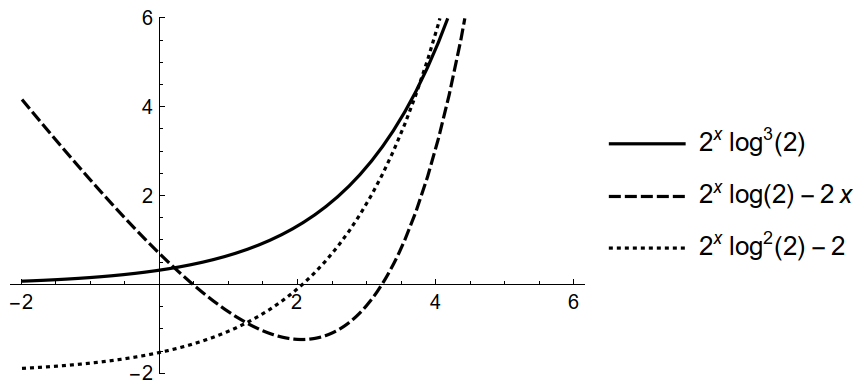
\includegraphics[width=0.5\textwidth]{figure/3-orders-dervatives-of-2-to-x---x-to2---1.png}
    \caption{The first, second and the third-ordered derivtives figures of $f(x)$ in Example \ref{ex:special-val-substitution}}
    \label{fig:3-orders-dervatives-of-2-to-x---x-to2---1}
\end{figure}

这种题型也比较喜欢和参数一起出,
这种情况应当先分离参数,比如\cite[page 77, pdf 88, 例5]{we}。
参数分离后往往对参数的讨论就会被延后,这样需要讨论的情况就会相对来说少很多。

进一步可参考:
\begin{itemize}
    \item \cite[page 85, pdf 96, example 6]{we}.
\end{itemize}

\subsection{(隐函数求)极值点}

可以参考 \cite[page 71, pdf 82, 例2]{we}.
此类问题可先对等式两边求导,之后 let $y' = 0$ 解出 $y$,
针对不同的 y 的解,结合题目要求进行验证排除不符合要求的选项。
之后再将符合要求的$y$ 带入原方程中, 这样就可以得到一个只含有一个参数$x$的函数了。
对于任何一种求极值点的问题,\textbf{都要应用其充分条件进行验证}。

其中,上文提到的各充分条件和必要条件请参考
\cite[page 68, pdf 79]{we}。

\subsection{证明函数不等式}

详情参阅 \cite[page 79, pdf 90]{we}

方法:
\begin{itemize}
    \item 单调性(最常用)
    \item 最大最小值
    \item Lagrange Mean Value Theorem
    \item Tylor Formula, 函数不等式往往考察函数的全局性质,从而需要使用拉格朗日余项。
    \item 函数的凹凸性
\end{itemize}

\subsection{微分中值定理的证明}

本部分内容难度比较大,应当结合\cite{we}进行复习。

题型:
\begin{itemize}
    \item $F\left[\xi, f'(\xi), f''(\xi)\right] = 0$.
        \begin{itemize}
            \item 分析法(还原)
            \item 微分方程法
            \item 常用辅助函数法
        \end{itemize}
    \item $F\left[\xi, \eta, f'(\xi), f'(\eta), f''(\xi), f''(\eta)\right] = 0$.
        \begin{itemize}
            \item 不要求 $\xi \neq \eta$
            \item 要求 $\xi \neq \eta$
        \end{itemize}
    \item $F\left[\xi, f^{(n)}(\xi)\right] \leq 0, (n \leq 2)$.
        \begin{itemize}
            \item Tylor\ref{tylor} 展开(Lagrange 余项), 
                  $x_0$ 选择函数值导数值提供信息多的点.
        \end{itemize}
\end{itemize}

\subsubsection{第一类题型}

通过上述三种方法找到辅助函数然后使用罗尔定理推出
\[
    \exists \xi \in \left(a, b\right), F'(\xi) = 0.
\]
其中,$F'(\xi)$ 直接作为提干中给出条件的式子,
但是还有一种情况是作为题干中式子的一个 factor.
如果是后者,则应当对 $F'(x)$ 的解析式进行说明,
以便推导出 $F'(x) = 0 \Rightarrow \mbox{原式子成立}$.
例题请参见 \cite[page 82, pdf 93, example 2]{we} 等.

常见的辅助函数请参见 \cite[page 83, pdf 94]{we}.
其中有一条比较 general 的:
\begin{align*}
    \mbox{欲证}\quad f'(\xi) + g(\xi) f(\xi) = 0,  \\
    \mbox{let} \quad 
    F(x) = \exp \left\{\int g(x) \mbox{d}x\right\} f(x).
\end{align*}

\section{好题收录}

\begin{example}
    武忠祥每日一题278\footnote{\url{https://www.bilibili.com/video/BV1zj411z71E}}.
    \begin{enumerate}
        \item 证明:$(1-x^2) y^{(n+1)} - (2n+1) xy^{(n)} - n^2 y^{(n - 1)} = 0 (n \geq 1)$
        \item 求 $y^{(n)}(0)$
    \end{enumerate}
\end{example}

\begin{example} \label{general-app-of-deritative-example}
    函数 $y = \dfrac{(x-3)^2}{4(x-1)}$ 的单调增区间是\underline{\quad\quad}, 
    单调减区间是 \underline{\quad\quad}, 极值是 \underline{\quad\quad}, 凹凸区间是\underline{\quad\quad}.

    \begin{center}
    \raisebox{0.5ex}{\rule{\textwidth}{0.3pt}}
    \end{center}

    方法:
    \begin{enumerate}
        \item 对函数进行变形,便于后续求导
        \item 求导
        \item 画表
    \end{enumerate}
    \cite[page 21, question 43]{w660ans}
\end{example}
例题 \ref{general-app-of-deritative-example}
中的函数 $y$ 可以变形为
\[
    y = \dfrac{x-1}{4} - 1 + \dfrac{1}{x-1}
\]
则
\begin{align}
    y' &= \dfrac{1}{4} - \dfrac{1}{(x-1)^2} \label{eq:deritative-for-further-defierentiation}\\
       &= \dfrac{(x-3)(x+1)}{4(x-1)^2}      \label{eq:deritative-for-finding-critical-point}
\end{align}
上述两个式子都是 $y'$, 但是其中 \ref{eq:deritative-for-further-defierentiation} 适合下一步求二阶导,
\ref{eq:deritative-for-finding-critical-point} 适合找驻点。

下一步就是画表
\footnote{这种题目\textbf{不会出大题},不用顾虑怎么在答题纸上表达啊这个表},
在这里因为篇幅关系就不绘图了
\footnote{希望有看到的人能帮忙提PR}。
可以简单说一下这个表的样子,首先表头被三个驻点分隔,
三个驻点两侧和中间是以它们为界的区间。
之后分别在这些驻点和区间上求函数的增减性、
凹凸性和函数值\footnote{为了求极值}即可。


